\documentclass[12pt]{exam}
\newcommand{\hwnumber}{6 \& 7}
\newcommand{\hwname}{Text Editor}
\newcommand{\duedate}{\formatdate{17}{10}{\YEAR} % day-month-year
  and\\\phantom{\textbf{Due: }}\formatdate{24}{10}{\YEAR} by \progDueTime}

\usepackage{../misc/latex/edition}  % Course semester
\usepackage{../misc/latex/c0}       % Listings style for c0
\usepackage{amsmath}
\usepackage{enumerate}
\usepackage[normalem]{ulem}
\usepackage{verbatim}
\usepackage[left=1in, right=1in, top=1in, bottom=1in]{geometry}
\usepackage{graphicx}
\usepackage{hyperref}
\usepackage{tikz}     \usetikzlibrary{shapes}
\usepackage{fancybox}
\usepackage[all]{xy}
\usepackage{wrapfig}
\usepackage{fancyvrb}
\usepackage{datetime}
\usepackage{etoolbox}
\usepackage{calc}
\usepackage[nomessages]{fp}
\usepackage{import}  % Like input and include, but respects subdirectories

\newcommand{\defaultQuestionLocation}{questions}
\newcommand{\inputQuestion}[2][\defaultQuestionLocation/]{%
  \subimport{#1}{#2}
}
% Subdirectories of \defaultQuestionLocation containing code and pictures
\newcommand{\code}{code}
\newcommand{\img}{img}


%%% ic: frontmatter macros
\newcommand{\specialInstructions}{}
\newcommand{\HWNUMBER}
{\ifdefempty{\hwnumber}{__}{%
  \ifnumless{\hwnumber}{10}{0\hwnumber}{\hwnumber}}}
\newcommand{\hwtype}{Written Homework}

%%% ic: 'exam' tweaks
\renewcommand{\half}{.5} % Half points

\newcommand{\Question}[2][]
 {\ifstrempty{#1}
    {\question{\bf #2}}
    {\question[#1]{\bf #2}}
  \immediate\write\rubricfile{}%
  \immediate\write\rubricfile{Question \thequestiontitle:}%
  \immediate\write\rubricfile{==========}
 }

%%% ic: Support for editable PDF
% counter name (some viewers misbehave if always the same)
\newcounter{editable}
\newcommand{\nextField}{\addtocounter{editable}{1}q\arabic{editable}}
\newcommand{\NextField}
 {\makebox[0pt][r]{\scalebox{0.1}{\color{White}\nextField}}}

% Color of edit area
\newcommand{\editAreaColor}{red}
% Single line answer:   \editableLine[extra parameters (optional)]{line width}
\newcommand{\editableLine}[2][]
{\textcolor{\editAreaColor}{%
 \underline{\hspace*{-0.25em}%
 \raisebox{-0.5ex}{%
 \TextField[width=#2, borderwidth=0, #1]{\NextField}}}}%
}
% Single line answer for code:  \editableLine[extra parameters (optional)]{line width}
\newcommand{\editableCodeLine}[2][]
{\textcolor{\editAreaColor}{%
 \underline{%
 \TextField[width=#2, height=1.5ex, borderwidth=0, #1]{\NextField}}}}
% Multiline answer:  \editableLine[extra parameters (optional)]{box height}
\newcommand{\editableBox}[2][]
{\leavevmode\hspace*{-0.1em}%
\TextField[height=#2, width=\linewidth,
           multiline=true, borderwidth=0.1, bordercolor=\editAreaColor,
           #1]{\NextField}}

%%%%% Same answer format as exams
\renewcommand{\rmdefault}{ppl}
\renewcommand{\sfdefault}{phv}
\newcommand{\answerColor}{Blue}

\ifprintanswers
\newcommand{\answer}[2]{\makebox[#1][c]{\color{\answerColor}#2}}
\else
\newcommand{\answer}[2]{\makebox[#1][c]{}\makebox[0pt]{\phantom{|}}}
\fi
\newcommand{\uanswer}[2]{\underline{\answer{#1}{#2}}}


%%% Write rubric snippet.  Usage:
% \RUBRIC
% any multi-line text (including \, #, %, whatever)
% ENDRUBRIC
%% (ENDRUBRIC should be on a line by itself)
\makeatletter
\def\RUBRIC
 {%
  \begingroup
  \let\do\@makeother\dospecials
  \endlinechar=`\^^J
  \@tofile%
 }
\def\ENDRUBRIC{ENDRUBRIC}
\def\@tofile#1^^J{%
  \def\@test{#1}%
  \ifx\@test\ENDRUBRIC
    \immediate\write\rubricfile{}  % End with an empty line
    \expandafter\@firstoftwo
  \else
    \expandafter\@secondoftwo
  \fi
  {\endgroup}%
  {\toks@{#1}%
   \begingroup\endlinechar=\m@ne
   \everyeof{\noexpand}%
   \xdef\@temp{\scantokens\expandafter{\the\toks@}}%
   \endgroup
   \immediate\write\rubricfile{\@temp}%
   \@tofile}%
}
\makeatother

%% Displays tags for an exercise in 'answer' mode
\newcommand{\TAGS}[1]
{\ifprintanswers%
  \rule{0em}{0ex}%
  \marginpar{\footnotesize%
    \fcolorbox{black}{Gray!25}{%
      \parbox[t]{2cm}{\raggedright\textbf{TAGS:}\\#1}}}%
  \ignorespaces%
 \fi}%


%% Page layout
\pagestyle{headandfoot}

\headrule
\header{\textbf{\courseNumber{} \hwtype{} \hwnumber}}
       {}
       {\textbf{Page \thepage\ of \numpages}}
\footrule
\footer{}{}{\COPYRIGHT}

\renewcommand{\partlabel}{\textbf{\thequestion.\thepartno}}
%\renewcommand{\partlabel}{\textbf{Task \thepartno}}
\renewcommand{\subpartlabel}{\textbf{\thesubpart.}}
\renewcommand{\thepartno}{\arabic{partno}}
\renewcommand{\thesubpart}{\alph{subpart}}
\pointpoints{pt}{pts}
\pointformat{\raisebox{0ex}[\height][0pt]{\fcolorbox{black}{yellow}{\themarginpoints}}}
\bonuspointformat{\raisebox{0ex}[\height][0pt]{\fcolorbox{black}{red}{\themarginpoints}}}
\marginpointname{\points}
\pointsinmargin
%\boxedpoints

\setlength\answerlinelength{2in}
\setlength\answerskip{0.3in}

\newcommand{\mkWrittenTitle}[1]{#1}
\newcommand{\mkDueDate}[1]{#1}
\newcommand{\mkEvalSummary}[1]{#1}
\newcommand{\mkGradetable}[1]{#1}



% This fixes an issue with the exam package version 2.6 and after,
% where 'framed' has been renamed to 'examframed' to avoid a conflict.
\ifcsmacro{examframed}{%
\newenvironment{framed}
{\begin{examframed}}
{\end{examframed}}
}{}

\begin{document}
\hwTitle

\noindent
For the programming portion of this week's homework, you'll implement
the core data structure for a text editor: the gap buffer. There are
\emph{two} deadlines: the first one is to make sure you've started,
and will give you your first 16 points on the assignment, which must be
earned at this time. The full
autograder will re-run the tests from the first part of the
assignment, but will not award points.  \emph{The checkpoint
  represents much less than half the assignment in terms of both lines
  of code and conceptual difficulty.}

\bigskip
\noindent
The code handout for this assignment is at
\begin{center}
\whereisthetgz{editor-handout.tgz}
\end{center}
The file \lstinline'README.txt' in the code handout goes over the
contents of the handout and explains how to hand the assignment
in. There is a FIVE (5) PENALTY-FREE HANDIN LIMIT for the checkpoint,
and another TEN (10) PENALTY-FREE HANDIN LIMIT for the second half of
the assignment. Every additional handin will incur a small (5\%)
penalty (even if using a late day). It is advisable to budget a few
handins specifically to get feedback on your specification functions;
having good specification functions will help you as you write the
rest of your code.

\paragraph{Style Grading:}
With this assignment, we will again emphasize \emph{programming style}
more heavily. We will actually be looking at your code and evaluating
it based on the criteria outlined at
\url{http://cs.cmu.edu/~15122/misc/styleguide.pdf}. We will make
comments on your code via Autolab, and will assign an overall passing
or failing style grade. A failing style grade will be
\emph{temporarily} represented as a score of -20 on the second part of
the assignment.  This -20 will be reset to 0 once you:
\begin{enumerate}
\itemsep=-3pt
\item%
  fix the style issues,
\item%
  see a member of the course staff during office hours \textbf{within
    5 days} after the grades are released, and
\item%
  briefly discuss the style issues and how they were addressed.
\end{enumerate}
We will evaluate your code for style in two ways. We will use
\lstinline'cc0' with the \lstinline'-w' flag that gives style warnings
--- code that raises warnings with this flag is almost certain to fail
style grading.  Because the \lstinline'-w' flag does not check for
good variable names, appropriate comments, or appropriate use of
helper functions, these issues will be checked by hand.

\paragraph{Contract Grading:}
Ten (10) points of this assignment will be given for writing good
contracts, as discussed further below.  Contracts will be graded by
hand after the final deadline as they cannot be checked by the
autograder.  Contract points count towards the second part of this
assignment, but they will be assessed over your overall code
(including the portions pertaining to the checkpoint).  Differently
from style points, contract points cannot be fixed after the final
deadline by going to a TA\@.  Points aside, good contracts will make
completing this assignment correctly \emph{much faster}.

Be sure to include the preconditions, postconditions and, where
necessary, loop invariants to ensure the data structure invariants and
the safety of your code.  More details about contracts are given
below.


\section{Overview: A text editor based on gap buffers}
\label{sect:overview}

In this assignment you will implement a simple text editor based on
the \emph{gap buffer} technique.  A gap buffer is a generalization
of an unbounded array: although an unbounded array allows for
efficient insertion and deletion of elements from the end, a gap
buffer allows for efficient insertion and deletion of elements in
the middle.

Given an unbounded array that is only half filled, adding items after
the last item currently in the array requires very little work,
because this simply means placing it in the next unused index and
increasing the \lstinline'size'. However, there is no unused space in
the middle. The only way to place a new item in the middle is to shift
elements over to make room for the new item.

A gap buffer attempts to avoid the cost of shifting by placing the
empty portion of the array somewhere within the array. Hence the name
``gap buffer'' referring to the ``gap'' within the
``buffer''. The gap is not fixed to any one position. At any time it
could be at the halfway point of the buffer or just at the beginning or
anywhere in the buffer. We can immediately see the potential benefits
of this approach.

When the user moves the \textbf{cursor} in the text editor, the
implementation automatically moves the gap, thereby providing the
unused portion of the array to be used for possible insertions. In the
worst case scenario we have to move the gap from the beginning of the
text file to the end. But if subsequent operations are only a few
indexes apart, we will get a lot better performance compared to using
a dynamic array. This is why it is said that the gap buffer technique
increases performance of repetitive operations occurring at relatively
close indexes. We claim without proof that the amortized cost of
insertion into the gap buffer is constant.

Implementing a text editor as just one gap buffer is not particularly
realistic. One large edit buffer requires the entire file contents to
be stored in a single, contiguous block of memory, which can be
difficult to allocate for large files. Instead, a more realistic
strategy is to combine the gap buffer technique with a doubly linked
list. The benefit of a linked list is that it allows the file to be
split across several chunks of memory. Therefore, in this assignment
we will represent a text editor as a doubly linked list where each
node contains a specific size of gap buffer. The contents of a text
file represented in this way is simply the concatenation of the
contents of each gap buffer in the linked list.

\paragraph{Warning:}
In the course so far, we have only considered interfaces (like pixels,
stacks, queues, and dictionaries) that did not expose their internal
representation to the user and that were tested without knowledge of
the implementation (black-box testing). The data structures and
interfaces we implement for this assignment do expose their internal
representation to the client.

The expectation is that the client (who is sometimes the text editor,
and sometimes you!) will mostly use this representation to read
information, and they will usually not write to the data structures
themselves. However, they are allowed to manipulate the data
structures, and so we expose the data structure invariants (like
\lstinline'is_gapbuf') as part of the interface.

This means that your data structure invariants will need to be
\emph{very good}, and we will test them very thoroughly. They need to
permit anything permitted by the specification, and disallow everything
that is not allowed by the specification. One thing we will \emph{not}
require you to do in this assignment is circularity checking: we will
never test your data structures against a doubly linked list where you
can follow \lstinline'next' pointers forever without reaching
\lstinline'NULL' or one where you can follow \lstinline'prev' pointers
forever without reaching \lstinline'NULL'.


\section{Gap Buffer}
\label{sect:gap-buffer}

A gap buffer is an array of characters. The array is logically split
into two segments of text --- one at the beginning of the array, which
grows upwards, and one at the end which grows downwards. The space
between those two segments is called the \emph{gap}. The gap represents the
\textbf{cursor} in the editor.  To move the cursor forwards, you just
move the gap. To insert a character after the cursor, you place it at
the beginning of the gap. To delete the character before the cursor,
you just expand the gap.

To implement a gap buffer there is some information that we need to
keep track of. A gap buffer is represented in memory by an array of
elements stored along with its size (\lstinline'limit') and two
integers representing the beginning (inclusive, \lstinline'gap_start')
and end (exclusive, \lstinline'gap_end') of the gap (see
Figure~\ref{fig:gapbuf}).

\begin{lstlisting}[numbers=none, belowskip=0pt]
typedef struct gapbuf_header gapbuf;
struct gapbuf_header {
    int limit;          /* limit > 0                     */
    char[] buffer;      /* \length(buffer) == limit      */
    int gap_start;      /* 0 <= gap_start                */
    int gap_end;        /* gap_start <= gap_end <= limit */
};
\end{lstlisting}
\begin{figure}[t]
\centering
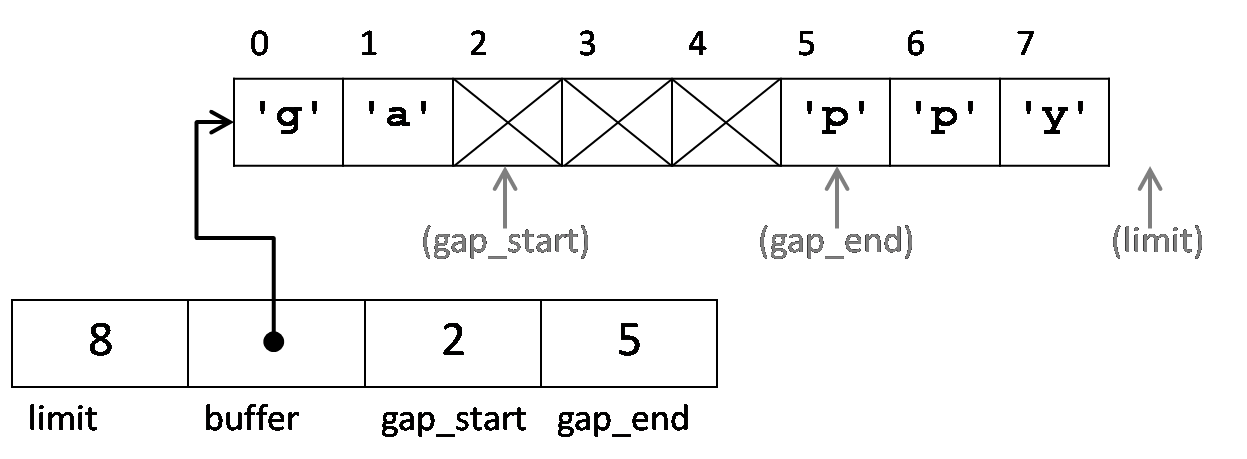
\includegraphics[width=0.75\textwidth]{\img/gapbuf.png}
\caption{A gap buffer in memory.}
\label{fig:gapbuf}
\end{figure}

\begin{task}[4]%[2]
\TAGS{array, ds-invariant}
A valid gap buffer is non-NULL, has a strictly positive limit which
correctly describes the size of its array, and has a gap start and
gap end which are valid for the array. Implement the function

\medskip
\lstinline'bool is_gapbuf(gapbuf* G)'
\medskip

\noindent%
that returns \lstinline'true' if \lstinline'G' satisfies the gap
buffer data structure invariants, and \lstinline'false' otherwise.
\end{task}

\enlargethispage{5ex}
Gap buffers may allow a variety of editing operations to be performed
on them; for the purposes of this assignment, we'll consider only four
operations: move forward a character, move backward a character,
insert a character, and delete a character. As an example, below is a
diagram of a gap buffer which is an array of characters with a gap in
the middle (situated between the ``p'' and the ``a'' in ``space''):
\begin{center} \lstinline"the sp[..]ace race" \end{center}\label{task3ref}


\noindent
To move the gap (the cursor in the text editor) forward, we copy a
character across it:
\begin{center} \lstinline"the spa[..]ce race" \end{center}

\noindent
To delete a character (before the cursor), we simply expand the gap:
\begin{center} \lstinline"the sp[...]ce race" \end{center}

\noindent
To insert a character (say, ``i''), we write it into the left side of
the gap (shrinking it by one):
\begin{center} \lstinline"the spi[..]ce race" \end{center}


\noindent
The gap can be at the left end of the buffer,
\begin{center} \lstinline"[..]the space race" \end{center}
or at the right end of the buffer,
\begin{center} \lstinline"the space race[..]" \end{center}
and a buffer can be empty,
\begin{center} \lstinline"[................]" \end{center}
or it can be full
\begin{center} \lstinline"the space ra[]ce!!" \end{center}
(some of these depend on the buffer size, i.e., \lstinline'limit').

\enlargethispage{1.5ex}

%\noindent
Note that in an Emacs-like interface, where the cursor appears as a
highlighted character in the buffer, the cursor will display on the
character immediately following the gap. So following the examples
above, \vspace{-5pt}
\begin{center} \lstinline"the sp[..]ace race" \end{center}
\vspace{-5pt}
would display as:
\vspace{-5pt}
\begin{center}
\begin{tikzpicture}
\draw (0.0,0) node{\large\texttt{the space race}};
\draw [line width=8] (-.12,-.3) -- (-.12,.32);
\draw (0.0,0) node{\large\texttt{\color{white}thespacerace~~~~~~a~~~~~~~thespacerace}};
\end{tikzpicture}
\end{center}
\vspace{-5pt}
while
\vspace{-5pt}
\begin{center} \lstinline"the space race[..]" \end{center}
\vspace{-5pt}
would display as:
\vspace{-5pt}
\begin{center}
\begin{tikzpicture}
\draw (0.0,0) node{\large\texttt{the space race}};
\draw [line width=8] (1.95,-.3) -- (1.95,.32);
\end{tikzpicture}
\end{center}
\vspace{-5pt}
%\begin{center} \lstinline"the space race "\;\lstinlineBox{\fbox}{\lstinline" "} \end{center}

In the above illustrations, we use dots to indicate spots in the gap
buffer whose contents we don't care about. Those spots in the gap
buffer don't need to contain the default character \lstinline|'\0'| or
the character \lstinline|'.'| or anything else in particular.


\begin{task}[6]%[3]
\TAGS{array, ds-invariant, safety}
Implement the following utility functions on gap buffers:

\begin{tabular}{p{0.45\textwidth}p{.45\textwidth}}
    \textbf{Function:}           & \textbf{Returns \lstinline'true' iff...}
\\ \lstinline"bool gapbuf_empty(gapbuf* G)"    & \ldots{t}he gap buffer is empty
\\ \lstinline"bool gapbuf_full(gapbuf* G)"     & \ldots{t}he gap buffer is full
\\ \lstinline"bool gapbuf_at_left(gapbuf* G)"  & \ldots{t}he gap is at the left end of the buffer
\\ \lstinline"bool gapbuf_at_right(gapbuf* G)" & \ldots{t}he gap is at the right end of the buffer
\end{tabular}
\end{task}


\begin{task}[6]%[3]
\TAGS{array, ds-invariant, safety}
Implement the following interface functions for manipulating gap buffers:

\begin{tabular}{p{0.5\textwidth}p{0.5\textwidth}}
  \lstinline"gapbuf* gapbuf_new(int limit)"     & Create a new gapbuf of size \emph{limit} \\
  \lstinline"void gapbuf_forward(gapbuf* G)"    & Move the gap forward, to the right \\
  \lstinline"void gapbuf_backward(gapbuf* G)"   & Move the gap backward, to the left \\
  \lstinline"void gapbuf_insert(gapbuf* G, char c)" & Insert the character $c$ before the gap \\
  \lstinline"void gapbuf_delete(gapbuf* G)"     & Delete the character before the gap
\end{tabular}
\end{task}

\smallskip\noindent
See page \pageref{task3ref} for details.
If an operation cannot be performed (e.g., moving the gap backward when
it's already at the left end), a contract (precondition) should fail.

All functions should require and ensure the data structure invariants.
Furthermore, the gap buffer returned by \lstinline"gapbuf_new" should be empty.
Use these facts to help you write your code, and document them with
appropriate assertions.

\subsection{Testing}

You can test your gap buffer implementation interactively by compiling
and running the provided \lstinline'gapbuf-test.c0'; you are encouraged
to use this file as a starting point for writing your own unit tests.

\begin{lstlisting}[language={[coin]C}]
 % cc0 -d -w -o gapbuf-test gapbuf.c0 gapbuf-test.c0
 % ./gapbuf-test
\end{lstlisting}
Try entering
``\lstinline'space race<<<<<<<<^p<<the >>^p>>>>>>>>!!<<<<<<<^^^^^great'''
and seeing what happens. (It is okay to share strings like this on
\qatool.)

\enlargethispage{5ex}
\begin{framed}\bf\noindent
After you have tested your gap buffer implementation, you can hand it
in before the checkpoint deadline to earn your first 16 points of the
assignment. No further points will be awarded for these tasks after
the checkpoint deadline.
\end{framed}

\clearpage
\begin{task}[10]
\TAGS{correctness, loop-invariant, safety}
  Be sure to include comprehensive contracts in all your code:
  preconditions, postconditions, and where necessary, loop invariants
  to ensure the data structure invariants and the safety of your
  code.  Please attach your contracts as part of the implementation of
  your functions, not their prototype.  This will be graded by hand
  after the final submission deadline.
\end{task}


\section{Doubly-Linked Lists}
\label{sect:text-buffer}

Another data structure that will be used to represent an edit buffer
is a \emph{doubly-linked list with a point}.  We have seen
singly-linked lists used to represent stacks and queues --- sequences of
nodes, each node containing some data and a pointer to the next node.
The nodes of a doubly-linked list as we will use them in this
assignment contain a \lstinline'data' field just like those of a
singly-linked list, but in contrast, the doubly-linked nodes contain
\emph{two} pointers: one to the next element (\lstinline'next') and one
to the \emph{previous} (\lstinline'prev').




\begin{figure}[ht]
\centering
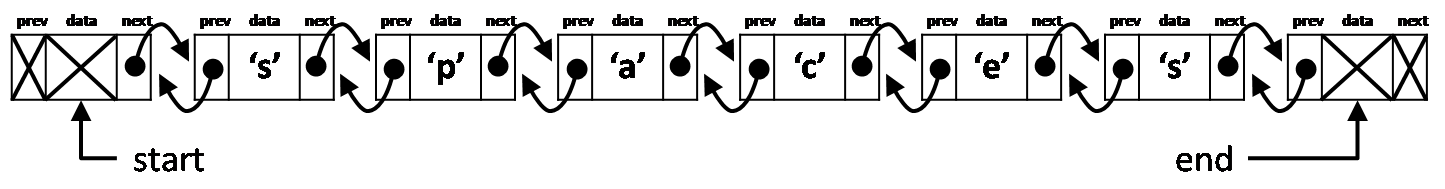
\includegraphics[width=0.75\textwidth]{\img/dll1.png}
\caption{An editable sequence as a doubly-linked list in memory.}
\label{fig:dll}
\end{figure}

An editable sequence is represented in memory by a doubly-linked list
and three pointers: one to the \lstinline'start' of the sequence, one
to the \lstinline'end' of the sequence, and one to the distinguished
\lstinline'point' node where updates may take place (see
Figure~\ref{fig:dll}).  We employ our usual trick of terminating the
list with ``dummy'' nodes whose contents we never inspect.

\medskip
\noindent
\begin{minipage}{0.4\linewidth}
\begin{lstlisting}
typedef struct dll_node dll;
struct dll_node {
    elem data;
    dll* next;
    dll* prev;
};
\end{lstlisting}
\end{minipage}
\hfill\rule[-8.5ex]{0.01em}{16.5ex}~
\begin{minipage}{0.55\linewidth}
\begin{lstlisting}
typedef struct dll_pt_header dll_pt;
struct dll_pt_header {
    dll* start;
    dll* point;
    dll* end;
};
\end{lstlisting}
\end{minipage}

\medskip
We can visualize a doubly-linked list as the sequence of its
\lstinline'data' elements with terminator nodes at both ends and one
distinguished element, called \lstinline'point':
\begin{center}
\lstinline"START <--> 'a' <--> " \fbox{\lstinline"'b'"} \lstinline" <--> END"
\end{center}
For now, we do not concern ourselves with the type of the
\lstinline'data' elements: basic doubly-linked list functions are
agnostic to it anyway.  (The picture above treats the data elements as
C0~characters.)


\newpage
\begin{task}[5]%[4]
\TAGS{ds-invariant, linked-list, pointer}
A valid doubly-linked list has the following properties:
\begin{itemize}
\item%
  the \lstinline'next' links proceed from the \lstinline'start' node
  to the \lstinline'end' node, passing the \lstinline'point' node along
  the way
\item%
  the \lstinline'prev' links mirror the \lstinline'next' links
\item%
  \lstinline'point' is distinct from both the \lstinline'start' and
  the \lstinline'end' nodes, i.e., the list is non-empty
\end{itemize}
Implement the function

\medskip
\lstinline'bool is_dll_pt(dll_pt* B)'
\medskip

\noindent%
that returns \lstinline'true' if \lstinline'B' satisfies the data
structure invariants of doubly-linked list with a point, and
\lstinline'false' otherwise.

You may find that writing a helper function %
\lstinline'bool is_dll_segment(dll* a, dll* b)' %
will help you implement
\lstinline'is_dll_pt'. You are not required to check for circularity, but
you may find it to be a useful exercise (it's actually easier for a
doubly linked list than for singly-linked ones).
\end{task}

\enlargethispage{5ex}

This task is not trivial. There are many ways for a doubly-linked list
to be invalid, even without circularity. For instance, your
\lstinline'is_dll_pt' function will be tested against structures with
\lstinline'NULL' pointers in various locations and against
almost-correct doubly-linked lists:
%like the ones in Figures~\ref{fig:dll2} and~\ref{fig:dll3}:

\begin{figure}[hb]
\centering
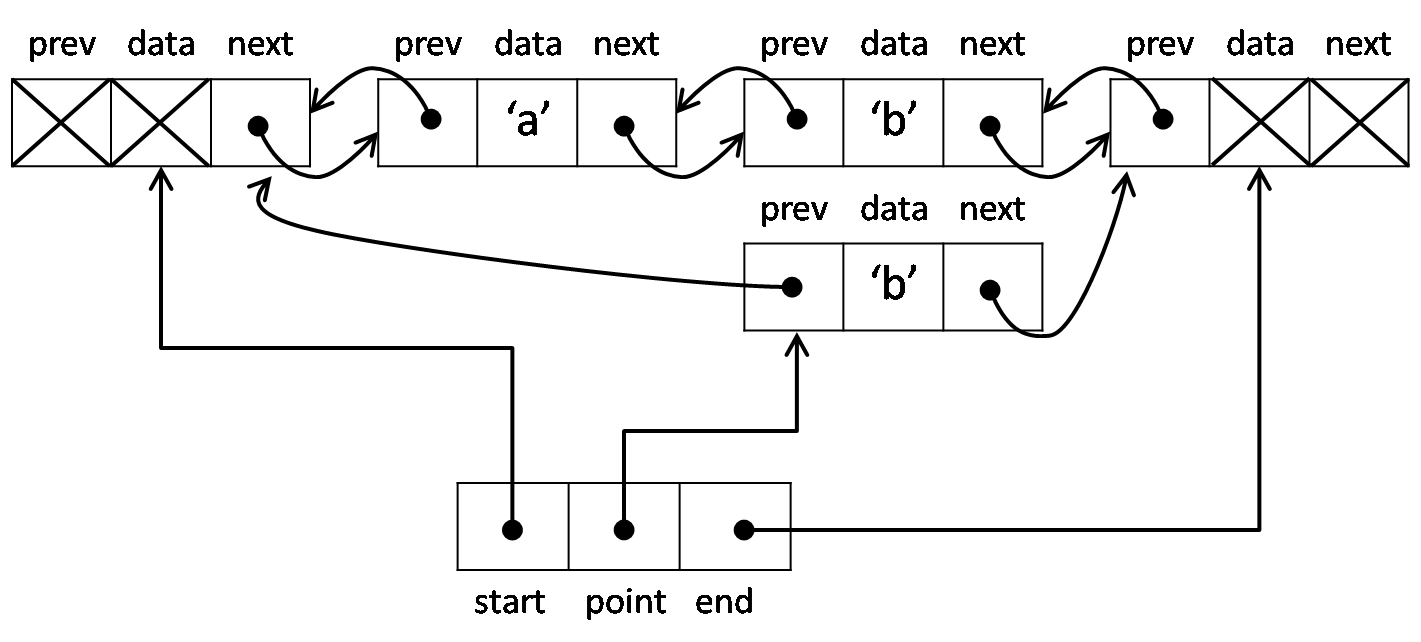
\includegraphics[width=0.7\textwidth]{\img/dll2.png}
\caption{Not a doubly-linked list (the \lstinline'point' isn't on the path
  from \lstinline'start' to \lstinline'end').}
\label{fig:dll2}
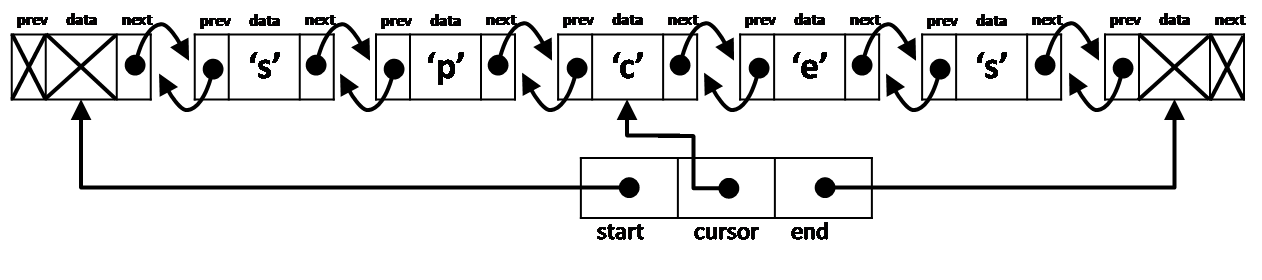
\includegraphics[width=0.7\textwidth]{\img/dll3.png}
\caption{Not a doubly-linked list (the \lstinline'prev' links don't
  mirror the \lstinline'next' links).}
\label{fig:dll3}
\end{figure}


\clearpage
\begin{task}[4]%[3]
\TAGS{ds-invariant, linked-list, pointer}
Implement the following utility functions on doubly-linked lists with points:

\medskip
\begin{tabular}{p{0.44\textwidth}p{.55\textwidth}}
   \textbf{Function:}
 & \textbf{Returns \lstinline'true' iff...}
\\[0.5ex]
   \lstinline"bool dll_pt_at_left(dll_pt* B)"
 & \ldots{t}he point is at the far left end
\\ \lstinline"bool dll_pt_at_right(dll_pt* B)"
 & \ldots{t}he point is at the far right end
\end{tabular}

\medskip
\noindent
and the following interface functions for manipulating doubly-linked
lists with points:

\medskip
\begin{tabular}{p{0.45\textwidth}p{.55\textwidth}}
   \lstinline"void dll_pt_forward(dll_pt* B)"
 & Move the point forward, to the right
\\ \lstinline"void dll_pt_backward(dll_pt* B)"
 & Move the point backward, to the left
\\ \lstinline"void dll_pt_delete(dll_pt* B)"
 & Remove the point node from the list
\end{tabular}
\end{task}

If an operation cannot be performed, a contract
(precondition) should fail.  When deleting the point, the new point
may be either to the right or to the left of the old one.

These functions should require and preserve the data structure
invariant you wrote above, and you should both document this fact and
use it to help write the code.  Be especially careful when
implementing deletion! Note, we cannot delete the point if it is the
only non-terminator node.

\subsection{Testing}

You can test your doubly-linked-list implementation interactively by
compiling and running the provided \lstinline'dll_pt-test.c0', which
treats elements as C0~characters as in the illustration
above. You are encouraged to use this file as a starting point for
writing your own unit tests.

\begin{lstlisting}[language={[coin]C}]
 % cc0 -d -w -o dll_pt-test elem-char.c0 dll_pt.c0 dll_pt-test.c0
 % ./dll_pt-test
\end{lstlisting}

Try entering ``\lstinline'steady''' as the input word and then
``\lstinline'^<<<<^>>^''' as the series of actions and seeing what
happens.

If you write your own test code, make sure that you put either
\lstinline'gapbuf.c0' (which declares the type \lstinline'elem' to be
\lstinline'gapbuf') or \lstinline'elem-char.c0' (which declares the
type \lstinline'elem' to be \lstinline'char') on the command line
before \lstinline'dll_pt.c0'. If you try to compile your
\lstinline'dll_pt.c0' file without first defining what
\lstinline'elem' is, you will probably get an error from
\lstinline'cc0' that looks something like %
\lstinline|"expected a type name, found identifier 'elem'"|, %
because the C0 compiler assumes \lstinline'"elem"' is an identifier
unless you have already used a \lstinline'typedef' to explain to C0
that it is really a type name.



\clearpage
\section{Putting It Together}
\label{sect:text-editor}

Now we will implement the \emph{text buffers} used by our text editor
as a doubly-linked list of fixed-size gap buffers (each buffer is 16
characters long).  The contents of a text buffer represented in this
way is simply the concatenation of the contents of its constituent gap
buffers, in order from the \lstinline'start' to the
\lstinline'end'. The gap representing the text editor's cursor is the
particular gap at the linked list's \lstinline'point'.  To move the
cursor, we use a combination of gap buffer motion and doubly-linked
list motion:
\begin{quote}
\begin{tabbing}
\hspace{3em}
\= \phantom{\emph{move $\leftarrow$}:~}
\= \lstinline"** <--> jus[.....] <-->"\;\fbox{\lstinline"t[..]_jump"}\;\lstinline"<--> **"
\\[0.5em]
\> \emph{move $\leftarrow$}:~
\> \lstinline"** <--> jus[.....] <-->"\;\fbox{\lstinline"[..]t_jump"}\;\lstinline"<--> **"
\\[0.5em]
\> \emph{move $\leftarrow$}:~
\> \lstinline"** <-->"\;\fbox{\lstinline"ju[.....]s"}\;\lstinline"<--> [..]t_jump <--> **"
\end{tabbing}
\end{quote}


\subsection{Text buffer invariants}

There are a lot of invariants that we want to check in this
representation. Two very simple ones are that our text buffers should
be a valid linked list (\lstinline'is_dll_pt'), and each element in
the linked list should be a gap buffer (\lstinline'is_gapbuf').

Another invariant that arises from this representation is that a text
buffer must either be the empty text buffer consisting of a single
empty gap buffer like this:
\begin{center}
\lstinline"START <--> "\fbox{\lstinline"[................]"}\lstinline" <--> END"
\end{center}
or else all the gap buffers must be non-empty. Additionally, all the
gap buffers are themselves well-formed, and they all have the same
size, and the size is 16. (We used gap buffers of size 8 for
simplicity in some of the examples, but you must use 16 in your
implementation.)

Another important invariant is \emph{alignment}. It is easiest to
observe on larger cases:
\begin{center}\vspace{-2.5ex}
\lstinline[deletestring={[b]{'}}]"** <--> well_i[..] <--> sn't_[...] <--> "\fbox{\lstinline"this_[..]l"}\lstinline" <--> [.....]ong <--> **"
\end{center}
Notice that for all gap buffers to the left of the point, the gap is
on the right. Similarly, for all gap buffers to the right of the
point, the gap is on the left. We call this invariant alignment. If
alignment fails to hold, we will have a very hard time moving the
point between gap buffers. If we had this text buffer instead:
\begin{center}\vspace{-2.5ex}
\lstinline[deletestring={[b]{'}}]"** <--> well_i[..] <--> sn't_[...] <--> "\fbox{\lstinline"this_[..]l"}\lstinline" <--> ong[.....] <--> **"
\end{center}
then, as we move to the right,
\begin{center}\vspace{-2.5ex}
\lstinline[deletestring={[b]{'}}]"** <--> well_i[..] <--> sn't_[...] <--> "\fbox{\lstinline"this_l[..]"}\lstinline" <--> ong[.....] <--> **"
\lstinline[deletestring={[b]{'}}]"** <--> well_i[..] <--> sn't_[...] <--> this_l[..] <--> "\fbox{\lstinline"ong[.....]"}\lstinline" <--> **"
\end{center}
we find that the cursor suddenly jumps to the end of the buffer,
skipping over ``ong'' entirely.

\begin{task}[4]
\TAGS{ds-invariant, linked-list}
A valid text buffer satisfies all the invariants
described above: it is a valid doubly-linked list containing valid
size-16 gap buffers, it is aligned, and it consists of either one
empty gap buffer or one or more non-empty gap buffers. Implement the
function

\medskip
\lstinline'bool is_tbuf(tbuf* B)'
\medskip

\noindent%
that returns \lstinline'true' if \lstinline'B' satisfies the text
buffer data structure invariants, and \lstinline'false' otherwise.
\end{task}

Hint: you may find it easier to decompose \lstinline'is_tbuf' into
multiple functions (such as one that checks alignment and one that
checks that the one-empty-or-all-nonempty property, etc).


\subsection{Manipulating text buffers}

\vspace{-\bigskipamount}
\begin{task}[2]%[1]
\TAGS{application, ds-invariant, linked-list}
Implement a text buffer constructor:

\begin{tabular}{p{0.3\textwidth}p{.7\textwidth}}
    \lstinline"tbuf* tbuf_new()       "  & Construct a new, empty text buffer
                                     with a \\
                                   & gap-buffer-size of 16
\end{tabular}
\end{task}

Recall that in order to be aligned, a text buffer must satisfy: all
gap buffers to the left of (``before'') the point must have their gaps
on the right, and all gap buffers to the right of (``after'') the
point must have their gaps on the left. Alignment specifies nothing
about the properties of the point itself.

To insert into the buffer (of the point node), we have to check if the
buffer is full or not.  When a gap buffer is full, we split the point
node into two nodes. The data in the buffer will be split as well:
\begin{quote}
\begin{tabbing}
\hspace{3em}
\= \phantom{\emph{insert `s'}:~}
\= \lstinline"** <-->"\;\fbox{\lstinline"splitend[]"}\;\lstinline"<--> **"
\\[0.5em]
\> \emph{insert `s'}:~
\> \lstinline"** <--> spli[....] <-->"\,\fbox{\lstinline"tends[...]"}\,\lstinline"<--> **"
\end{tabbing}
\end{quote}
\noindent
To split a full gap buffer, we have to copy each half of the character data
into one of two new gap buffers, taking special note of where the new gaps
should end up.  The following diagrams may help you visualize the intended
result:
\begin{center}
\begin{tabular*}{0.94\textwidth}{l@{\hspace{3em}}|@{\hspace{1em}}r}
%\begin{tabular*}{0.94\textwidth}{l@{\extracolsep{\fill}}r}
\begin{minipage}{0.47\textwidth}
\begin{tabbing}
\= \emph{full buffer:~} % \phantom{\emph{splits into:~}}
\= \fbox{\lstinline"abc[]defghABCDEFGH"} \\[1.0em]
\> \emph{splits into:~}
\> \fbox{\lstinline"abc[........]defgh"} \\
\> \>            \;\lstinline"[........]ABCDEFGH"
\end{tabbing}
\end{minipage}
&
\begin{minipage}{0.47\textwidth}
\begin{tabbing}
\= \emph{full buffer:~} % \phantom{\emph{splits into:~}}
\=   \fbox{\lstinline"stuvwxyzSTUV[]WXYZ"} \\[1.0em]
\> \emph{splits into:~}
\>                  \;\lstinline"stuvwxyz[........]"  \\
\> \> \fbox{\lstinline"STUV[........]WXYZ"}
\end{tabbing}
\end{minipage}
\end{tabular*}
\end{center}
We can then link the new gap buffers into the doubly-linked list, taking
care to preserve the text buffer invariants.


\begin{task}[4]%[3]
\TAGS{application, ds-invariant, linked-list, pointer}
Implement a function \lstinline"tbuf_split_pt(tbuf* B)" which takes a valid
text buffer whose point is full and turns it into a valid text buffer
whose point is not full. If you find it helpful to do so, you can
extend the interface to gap buffers or doubly-linked lists with
points as part of your solution.
\end{task}


To delete from the buffer we use the gap buffer's
\lstinline'gapbuf_delete' function. When one of the buffers becomes
empty, we delete it unless it is the only gap buffer left:
\begin{quote}
\begin{tabbing}
\hspace{3em}
\= \phantom{\emph{delete}:~}
\= \lstinline"START <--> deletio[.] <-->"\;\fbox{\lstinline"n[........]"}\;\lstinline"<--> END"
\\[0.5em]
\> \emph{delete}:~
\> \lstinline"START <-->"\;\fbox{\lstinline"deletio[.]"}\;\lstinline"<--> END"
\end{tabbing}
\end{quote}


\newpage
\begin{task}[5]%[4]
\TAGS{application, ds-invariant, linked-list}
Implement the following interface functions for manipulating text buffers:

\begin{tabular}{p{0.45\textwidth}p{0.5\textwidth}}
  \lstinline"void tbuf_forward(tbuf* B)"    & Move the cursor forward, to the right \\
  \lstinline"void tbuf_backward(tbuf* B)"   & Move the cursor backward, to the left \\
  \lstinline"void tbuf_insert(tbuf* B, char c)" & Insert the character $c$ before the cursor \\
  \lstinline"void tbuf_delete(tbuf* B)"     & Delete the character before the cursor
\end{tabular}

\medskip
\noindent
\textbf{These functions directly respond to a user's input.}  That
means that if an operation cannot be performed (e.g., pressing the
``left'' key to move the cursor backward with
\lstinline'tbuf_backward' when it's already at the left end), the
function should leave the text buffer \textbf{unchanged} instead of
raising an error or assertion violation.
\end{task}



\subsection{Testing}

You can test your text buffer implementation interactively by
compiling and running the provided \lstinline"tbuf-test.c0", which works
much like \lstinline'gapbuf_test.c0'. You are encouraged to use this file
as a starting point for writing your own unit tests.  The
\lstinline'README.txt' has some suggested inputs.

\begin{lstlisting}[language={[coin]C}]
 % cc0 -d -w -o tbuf-test gapbuf.c0 dll_pt.c0 tbuf.c0 tbuf-test.c0
 % ./tbuf-test
\end{lstlisting}

After you've completed your text buffer implementation and tested it
thoroughly, you can try it out interactively by compiling against
\lstinline"lovas-E0.c0" --- a minimalist text editor front-end written by
William Lovas.

\begin{lstlisting}[language={[coin]C}]
 % cc0 -d -w -o E0 gapbuf.c0 dll_pt.c0 tbuf.c0 lovas-E0.c0
 % ./E0
\end{lstlisting}

\noindent
Enjoy the hard-won fruits of your careful programming labors!

%% \section{Bonus: Extending the Editor}

%% Extend the E0 editor implementation with some interesting features. A
%% few suggestions to pique your imagination: a better display
%% algorithm, a better splitting algorithm, line motion, more editing
%% commands, copy and paste --- be creative! Feel free to extend the data
%% structures in any way necessary to support your changes
%% effectively. Submit your modified implementation as files named
%% \lstinline'bonus-*.c0' and include a \lstinline'bonus-README.txt' file
%% explaining your work and how it can be compiled. The entries will be
%% judged both in terms of the interactive editing experience, the
%% supporting data structures and algorithms, and the quality of the
%% code.

\clearpage
\section{Appendix: List of functions to implement}

To help you keep track of the large number of functions you're
writing, here's a list. Of course you may (should) define other helper
functions and extend these interfaces as appropriate.

\begin{lstlisting}[numbers=none, basicstyle=\smallbasicstyle, columns=fixed]
gapbuf.c0 - Gap buffers
  bool is_gapbuf(gapbuf* G);

  bool gapbuf_empty(gapbuf* G);       /* Returns true if the buffer is empty */
  bool gapbuf_full(gapbuf* G);        /* Returns true if the buffer is full  */
  bool gapbuf_at_left(gapbuf* G);     /* Returns true if the gap is at the
                                           left end of the buffer            */
  bool gapbuf_at_right(gapbuf* G);    /* Returns true if the gap is at the
                                           right end of the buffer           */
  gapbuf* gapbuf_new(int limit);      /* Create a new gapbuf of size limit   */
  void gapbuf_forward(gapbuf* G);     /* Move the gap forward, to the right  */
  void gapbuf_backward(gapbuf* G);    /* Move the gap backward, to the left  */
  void gapbuf_insert(gapbuf* G, char c); /* Insert char c before the gap     */
  void gapbuf_delete(gapbuf* G);      /* Delete the char before the gap      */

dll_pt.c0 - Doubly-linked lists with a point
  bool is_dll_pt(dll_pt* B);

  bool dll_pt_at_left(dll_pt* B);     /* Returns true if the point is first
                                           first (non-terminal) node         */
  bool dll_pt_at_right(dll_pt* B);    /* Returns true if the point is last
                                           last (non-terminal) node          */
  void dll_pt_forward(dll_pt* B);     /* Moves the point forward (right)     */
  void dll_pt_backward(dll_pt* B);    /* Moves the point backward (left)     */
  void dll_pt_delete(dll_pt* B);      /* Remove the current point            */

tbuf.c0 - Text buffers
  bool is_tbuf(tbuf* B);

  tbuf* tbuf_new();                   /* Creates an empty text buffer        */
  void tbuf_split_pt(tbuf* B);        /* Splits a full point into two nodes  */
  void tbuf_forward(tbuf* B);         /* Move the cursor forward/right by 1  */
  void tbuf_backward(tbuf* B);        /* Move the cursor backward/left by 1  */
  void tbuf_insert(tbuf* B, char c);  /* Insert the char before the cursor   */
  void tbuf_delete(tbuf* B);          /* Delete the char before the cursor   */
\end{lstlisting}

\end{document}
